\chapter{Aplikacje klienckie}

\section*{Aplikacja Android}

\section*{Aplikacja iOS}
Aplikacja przeznaczona jest na urządzenia z systemem operacyjnym iOS od wersji 10.0. 
Nie wspiera ona wcześniejszych wersji ze względu na nowe funkcje, które Apple wprowadziło wraz z pojawieniem się iOS 10.0 (m.in. klasa UNUserNotificationCenter). Jednak jak wynika z wykresu niżej (numer rysunku) 92\% wszystkich obecnych użytkowników tego systemu jest w stanie zainstalować aplikację a liczba ta z czasem stale rośnie. Aplikacja wspiera zarówno telefony komórkowe iPhone jak i tablety iPad. 
\begin{figure}[h]
	\centering
	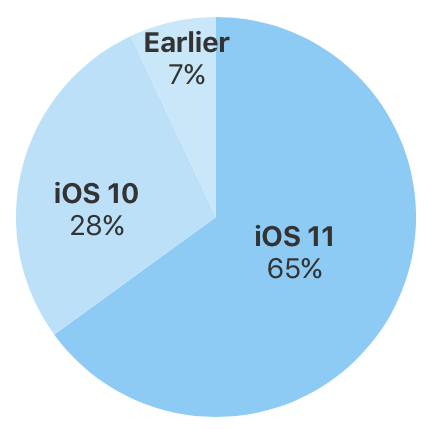
\includegraphics[width=6cm]{iOSstat}
	\caption{Udziały wersji systemu iOS w rynku}
\end{figure}
Napisana jest w stosunkowo nowym języku Swift (zaprezentowany przez Apple w 2014r na konferencji WWDC) w oparciu o architekturę MVC (Model-View-Controller) wykorzystując przy tym programowanie reaktywne i funkcjonalne. Aplikacja powstała w programie Xcode.
Programowanie reaktywne zrealizowano przy pomocy biblioteki RxSwift. Programowanie reaktywne związane jest z pojęciem obserwatora i sekwencji obserwowalnych. Każdy obserwator wywołując funkcję 'subscribe' na elemencie obserwowalnym otrzymuje informację o każdej zmianie na tym obiekcie. RxSwift wykorzystano m.in w celu wznowienia streamu obrazu z kamery w momencie przejścia aplikacji z trybu background do trybu foreground. Oznacza to, że po wyjściu z aplikacji, ale pozostawiając ja działającą w tle i po ponownym jej uruchomieniu traciliśmy obraz ze streamu. Przyczyną jest polityka Apple, która nie zaleca aby aplikacje pracowały w tle i domyślnie wyłącza każdą taką aktywność. Ma to na celu przedłużenie żywotności baterii i poprawie pracy całego systemu poprzez ograniczenie ilości zajmowanych zasobów [https://developer.apple.com/library/content/documentation/iPhone/Conceptual/iPhoneOSProgrammingGuide/BackgroundExecution/BackgroundExecution.html].  Oczywiście istnieje możliwość włączenia pracy w tle, jednakże konieczne jest aktywowanie trybu "Background Mode" i zaznaczenie konkretnej aktywności, którą chcielibyśmy wykonywać. Lista dozwolonych czynności możliwych do realizacji w tle jest ograniczona (rys x). 
\begin{figure}[h]
	\centering
	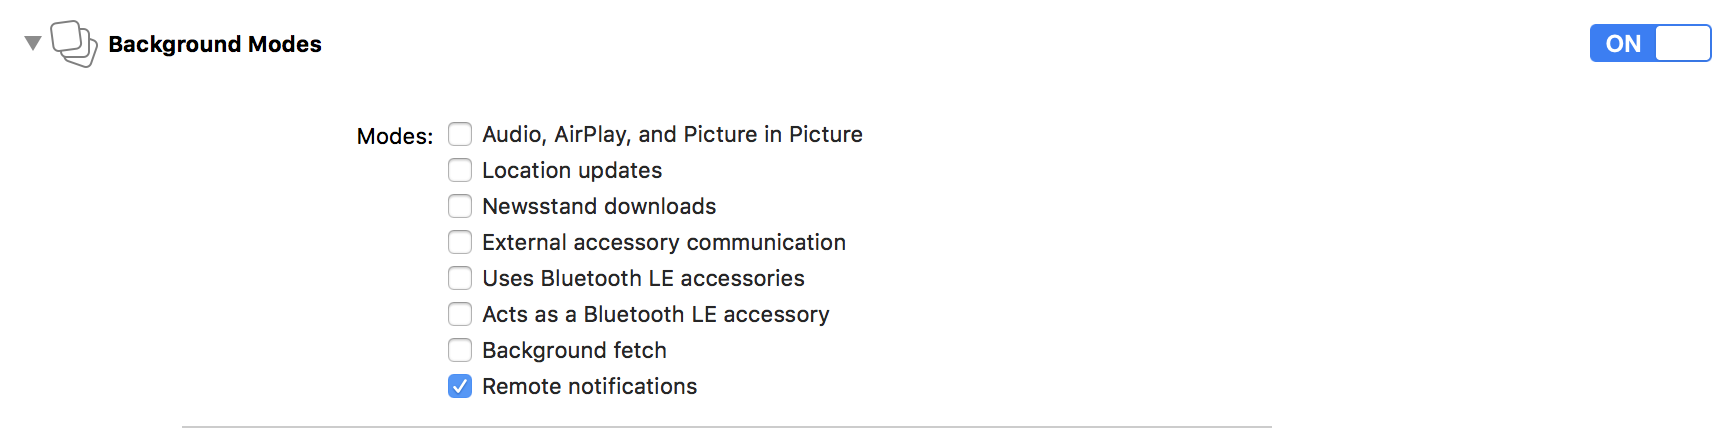
\includegraphics[width=9cm]{backgroundModes}
	\caption{Tryby pracy w tle}
\end{figure}
Próba oszustwa i wykonywania innej pracy w tle niż zaznaczona zostanie wychwycona w procesie weryfikacji przed jej publikacją na platformie Apple Store. Dzięki programowaniu reaktywnemu problem wznowienia podglądu obrazu został rozwiązany co prezentuje poniższy kod:
\begin{verbatim}
let appDelegate = UIApplication.shared.delegate as! AppDelegate
        appDelegate.inBackground.asObservable().subscribe(onNext: { (value) in
            if let streamView = self.streamView {
                if let player = self.currentPlayer {
                    if value == false {
                        self.streamVideoFrom(urlString: self.currentUrlString!)
                        print("Enter foreground")
                    } else {
                        print("Enter background")
                        streamView.layer.sublayers?.forEach({ (layer) in
                            layer.removeFromSuperlayer()
                        })
                    }
                }
            }
        }).disposed(by: disposeBag)
\end{verbatim}
Zmienna 'inBackground', która jest zmienną obserwowalną, ustawiana jest w oddzielnej klasie AppDelegate(klasa, która zapewnie poprawną interakcję z systemem iOS) na wartość true w chwili przejścia do trybu pracy w tle i na wartość false w przeciwnym wypadku. Klasa, w której wywoływany jest funkcja 'subscribe' jest obserwatorem tej zmiennej. Kod wewnątrz funkcji subscribe uruchamiany jest przy każdej zmianie wartości 'inBackground' i wznawia ponownie stream po każdym ponownym uruchomieniu programu.
"Programowanie funkcjonalne natomiast polega na traktowaniu funkcji jako obiektu. Oznacza to, że mogą być one zapisywane, kopiowane i przekazywane tak samo jak wszystkie inne obiekty. Mogą być używane jako parametry innych funkcji." [Pro Swift, Paul Hudson 04.19.2016 strona 172 link do store na iTunes : https://itunes.apple.com/us/book/pro-swift/id1111033310?mt=11 ]. Wykorzystane są w miejscach gdzie konieczne jest przekształcanie danych:
\begin{verbatim}
lastNotification = notifications.array.sorted(by: { (n1, n2) -> Bool in
	n1.date > n2.date 
}).filter({ (notif) -> Bool in return notif.type == "PIRSensor"}).first
\end{verbatim}
Na tablicy z notyfikacjami zastosowano szereg kolejnych funkcji: posortowano je malejąco według daty, przefiltrowano w taki sposób aby wybrać tylko te o typie 'PIRSensor' czyli te pochodzące z czujnika ruchu. Na sam koniec wybrano tylko jeden pierwszy element z wybranych i wynik wpisano do zmiennej lastNotification. Ważne jest, że każda kolejna wywoływana funkcja np. filter, odbiera wynik poprzedniej. 

Strukturę kodu(rys. 5.2) podzielono na kilka osobnych, logicznych części. Folder Firebase zawiera model bazy danych czujników, które zapisane są na serwerach Firebase. W folderze GuardManager znajdują się elementy odpowiedzialne za komunikację REST-ową z serwerem Django i modele bazy danych znajdującej się na naszym serwerze. Folder Views jest zbiorem widoków, które wczytywane są w zależności, w której sekcji się znajdujemy (opis sekcji niżej). ViewController.swift jest głównym kontrolerem zarządzającym widokami i modelami. Odpowiada za załadowanie odpowiedniego widoku i prezentację danych z odpowiedniej sekcji. W folderze GuardianAppTests napisane zostały testy jednostkowe, które sprawdzają poprawność przekształcania danych typu JSON (odpowiedź serwera) do obiektów zdefiniowanych w folderze GuardManager/Models. Klasy, których nazwy kończą się na Manager oznaczają obiekty typu Singleton. Celem takiego wzorca jest zapewnienie istnienia tylko jednej instancji w całej aplikacji i globalnego dostępu do tego obiektu. GuardManager, który odpowiada za pobieranie danych z bazy danych - taki obiekt nie powinien być utworzony więcej niż jeden raz, gdyż wszystkie klasy, które z niego korzystają nie potrzebują kolejnych instancji tej klasy. W ten sposób zapewniono, że zawsze odwołujemy się do tego samego obiektu.
\begin{figure}[h]
	\centering
	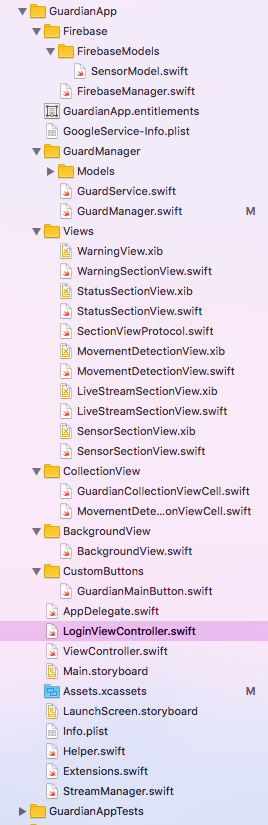
\includegraphics[width=4cm]{iOSstructure}
	\caption{Struktura aplikacji}
\end{figure}
Instalacja zewnętrznych bibliotek odbywa się za pomocą CocoaPods. Jest to menadżer zależności dzięki któremu szybko możemy wyszukać i zainstalować wymagane oprogramowanie. Wszystkie użyte zależności przedstawiono poniżej: 
\begin{verbatim}
  pod 'Moya'
  pod 'MBProgressHUD', '~> 1.0'
  pod 'RxSwift',    '~> 4.0'
  pod 'RxCocoa',    '~> 4.0'
  pod 'IHKeyboardAvoiding'
  pod 'Moya-SwiftyJSONMapper'
  pod 'Firebase/Core'
  pod 'Firebase/Messaging'
  pod 'Firebase/Auth'
  pod 'Firebase/Database'
  pod 'M13ProgressSuite'
\end{verbatim}
Moya używana jest do asynchronicznej REST-owej komunikacji z serwerem Django. SwiftyJSONMapper przydatna okazuje się do przekształcenia odpowiedzi serwera w postaci JSON do wcześniej zdefiniowanego modelu. MBProgressHUD umożliwia wyświetlanie ekranu ładowania podczas pobierania informacji z serwera. RxSwift i RxCocoa to biblioteki do programowania reaktywnego. Moduły Firebas/Core itp. służą do komunikacji z serwerami Firebase. Ostatni 'pod M13ProgressSuite' służy do rysowania wykresów i animowanych elementów graficznych w systemie iOS.
Po uruchomieniu aplikacji pierwszym widokiem jest ekran logowania i rejestracji użytkowników(rys 5.2). 
\begin{figure}[h]
	\centering
	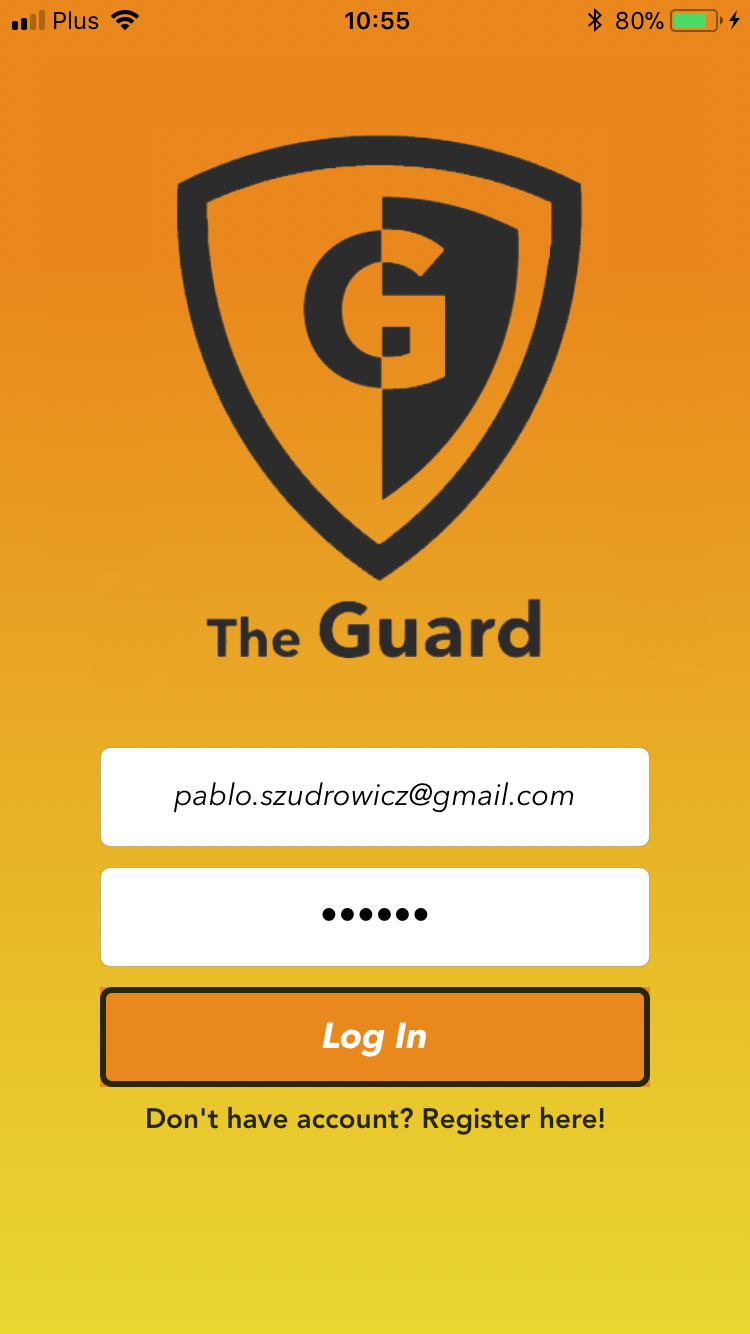
\includegraphics[width=5cm]{login.png}
	\caption{Ekran logowania}
\end{figure}
Po prawidłowym uwierzytelnieniu użytkownika uzyskiwany jest dostęp do głównego widoku aplikacji. W górnej części możliwy jest wybór 5 sekcji:
sekcja czujników, sekcja historii notyfikacji, sekcja ostatnich zagrożeń przy wykryciu ruchu, sekcja streamu na żywo, sekcja ustawień. Wszystkie te sekcje dotyczą konkretnego urządzenia wybranego w pasku na dole ekranu. Przy pierwszym uruchomieniu nie istnieje żadne urządzenie przypisane do naszego konta użytkownika. Aby dodać pierwsze i kolejne stacje, od których chcemy otrzymywać notyfikacje o zagrożeniach a także śledzić i monitorować informacje z czujników należy wybrać przycisk "New" z plusikiem w dolnej części ekranu. Pojawi się okno z prośbą o wpisanie numeru identyfikującego urządzenie. Po chwili dodany "Guard" będzie widoczny w na liście.
\paragraph{Sekcja czujników:}
Jest to jedna z najważniejszych sekcji aplikacji (rys 5.3).  Otrzymuje ona dane z czujników w czasie rzeczywistym i prezentuje je użytkownikowi.  W zależności od koloru prezentowanej wartości z czujnika użytkownik analizuje zagrożenie. Kolor zielony reprezentuje bezpieczne i prawidłowe odczyty na czujnikach, kolor pomarańczowy średnie, kolor czerwony reprezentuje bardzo wysoki poziom niebezpieczeństwa. Implementacja tej funkcjonalności zrealizowana została przy pomocy modelu HSV, który w przeciwieństwie do RGB pozwala na bardzo proste przejście z jednego koloru do kolejnego poprzez zmienę tylko jednego parametru. Zmieniając parametr Hue zmieniamy barwę przy stałym nasyceniu i jasności. Wartość tego parametru równa 120\textdegree{} odpowiada kolorowi zielonemu, kolor czerwony to 0\textdegree{}. Przekształcając wartość otrzymaną z czujników, która jest z zakresu [0-1] na wartość z przedziału [120-0] otrzymano wspomniany efekt. 
Poniżej przedstawiono fragment konwersji danych z czujników na kolor w modelu HSV, gdzie zmienna sensors[0] reprezentuje czujnik LPG.
\begin{verbatim}
UIColor(hue: CGFloat(0.33 - (sensors[0].value * 0.33)),
saturation: 1, brightness: 1, alpha: 1)
\end{verbatim}
\begin{figure}[h]
	\centering
	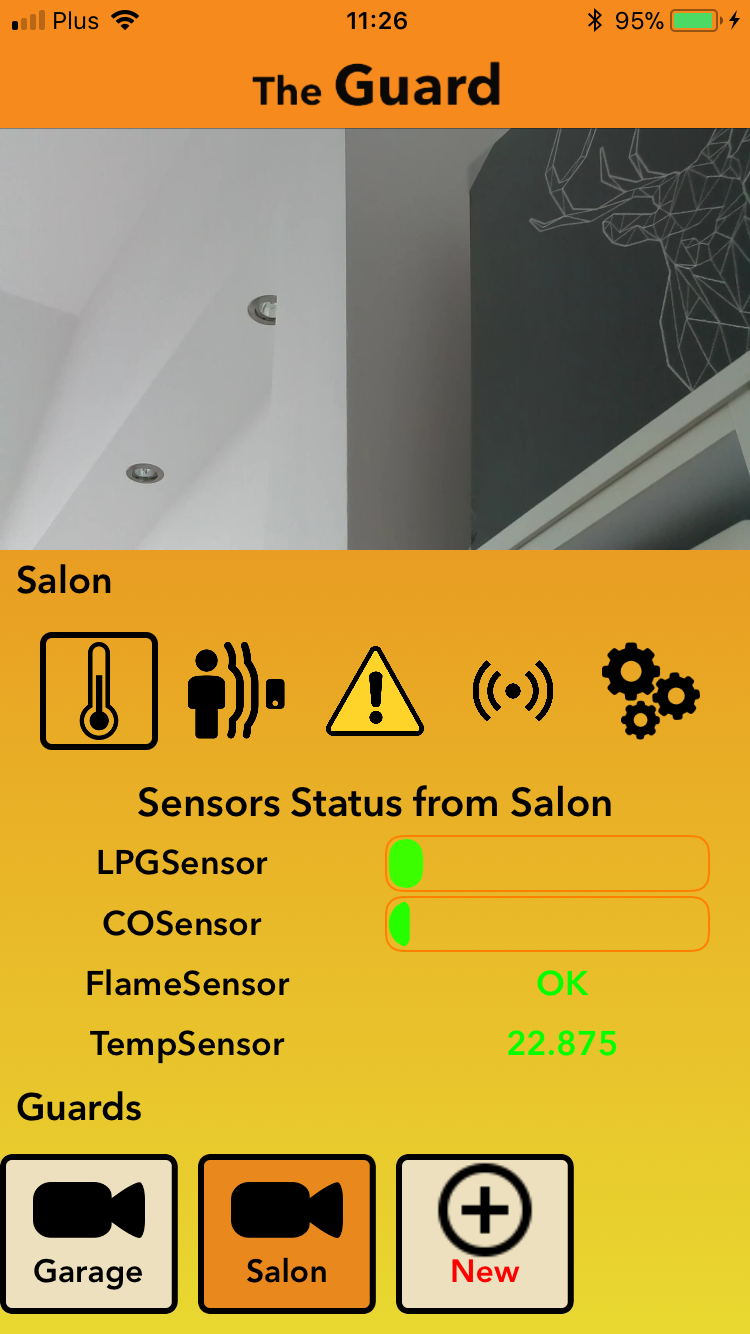
\includegraphics[width=5cm]{sensors.png}
	\caption{Sekcja czujników}
\end{figure}
\paragraph{Sekcja historii notyfikacji:}
W tej sekcji użytkownik ma dostęp do historii zdarzeń w systemie (rys 5.4). Po zaznaczeniu daty reprezentującej moment wystąpienia zagrożenia i wybranu przycisku 'preview' prezentowana jest informacja o miejscu niebezpieczeństwa i jego rodzaju. 
\begin{figure}[h]
\centering
\begin{minipage}{.4\linewidth}
    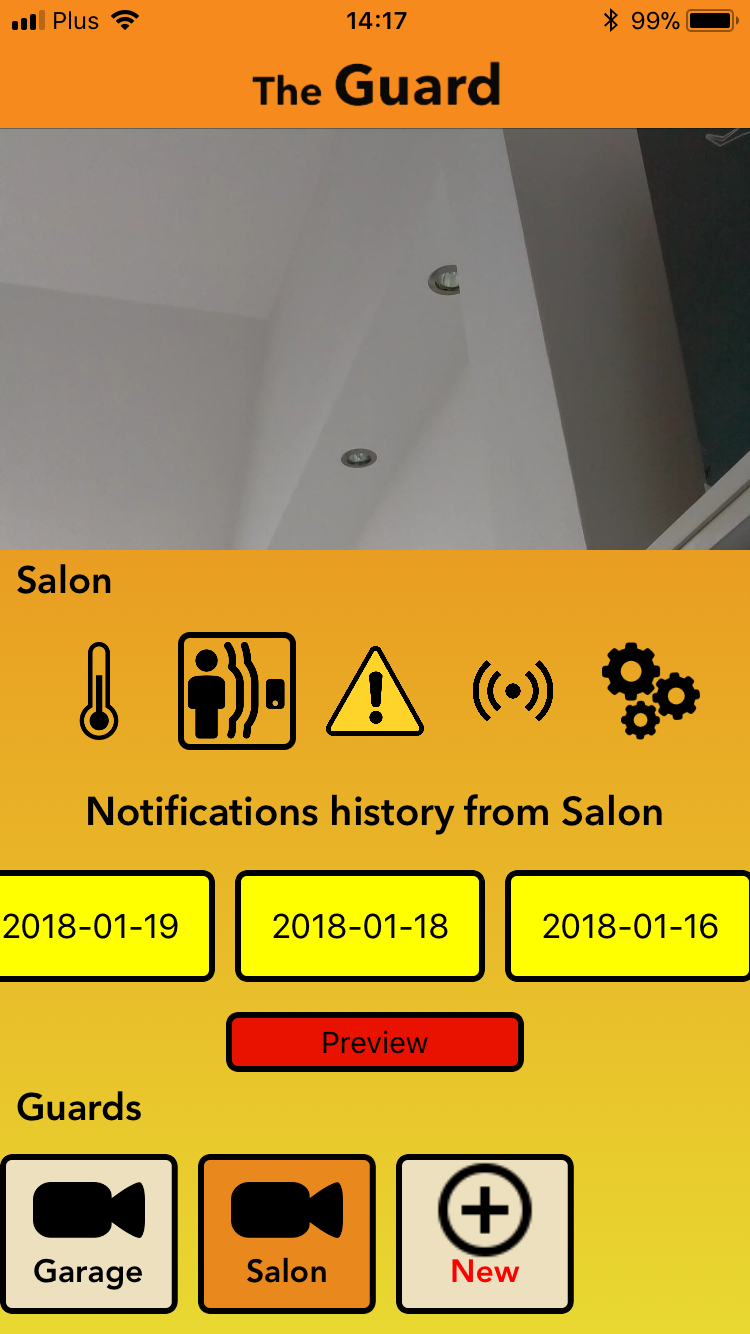
\includegraphics[width=\linewidth]{history.png}
    \caption{Sekcja historii notyfikacji}
    \label{img1}
\end{minipage}
\hspace{.05\linewidth}
\begin{minipage}{.4\linewidth}
    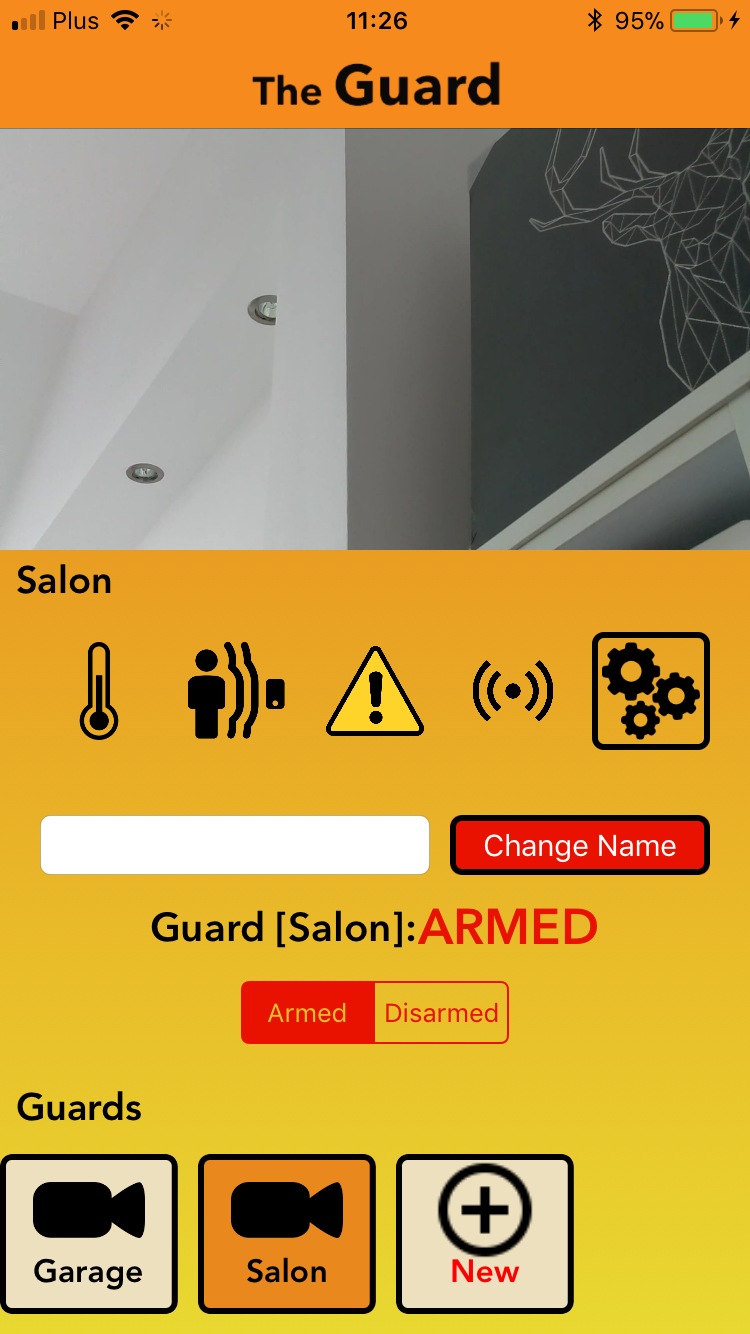
\includegraphics[width=\linewidth]{settings.png}
    \caption{Sekcja ustawień}
    \label{img2}
\end{minipage}
\end{figure} 
\paragraph{Sekcja ustawień:}
Użytkownik ma możliwość zmiany nazwy urządzenia, które zazwyczaj reprezentuje miejsce, w którym się znajduje. Istnieje również możliwość uzbrojenia i wyłączenia każdego urządzenia. Sprowadza się to do tego, że w przypadku zaznaczenia opcji "Disarmed" użytkownik nie otrzyma kolejnych notyfikacji o zagrożeniach. Opcja ta może okazać się przydatna w momencie uszkodzenia któregoś z modułów i tym samym błędnych danych wysyłanych z czujników.
\paragraph{Sekcja streamu:}
Sekcja odpowiedzialna za prawidłowy odbiór obrazu z kamery zaznaczonej w dolnej części ekranu. Okno, w którym odbywa się stream ustawiono w taki sposób, aby bez względu na rozmiar telefonu utrzymywało proporcję 16:9. Pozbyto się dzięki temu czarnych ramek lub braku części obrazu ze streamu.
\paragraph{Sekcja ostatnich zagrożeń:}
Sekcja prezentuje ostatnie nagrane zagrożenie. Służy do szybkiego przeglądu ostatniego niebezpieczeństwa i prezentuje ostatni nagrany materiał video. 

Przeprowadzono kilka testów aplikacji pod pełnym obciążeniem za pomocą programu Instruments. Szczególnie interesująco przedstawia się zużycie sieci podczas streamu obrazu. Widać, że w ciągu jednej minuty pobrano 6,61MB a wysłano jedynie 24,11Kb. Obraz pobierany jest tylko wtedy kiedy aplikacja jest aktywna. W ciągu godziny działania aplikacji pobierze ona około 400MB danych. Jednak dla zapewnienia komfortu użytkowania i płynnego streamu obrazu zalecane jest posiadanie łącza umożliwiającego transfer danych na poziomie min. 200KB/s. 
\begin{figure}[h]
	\centering
	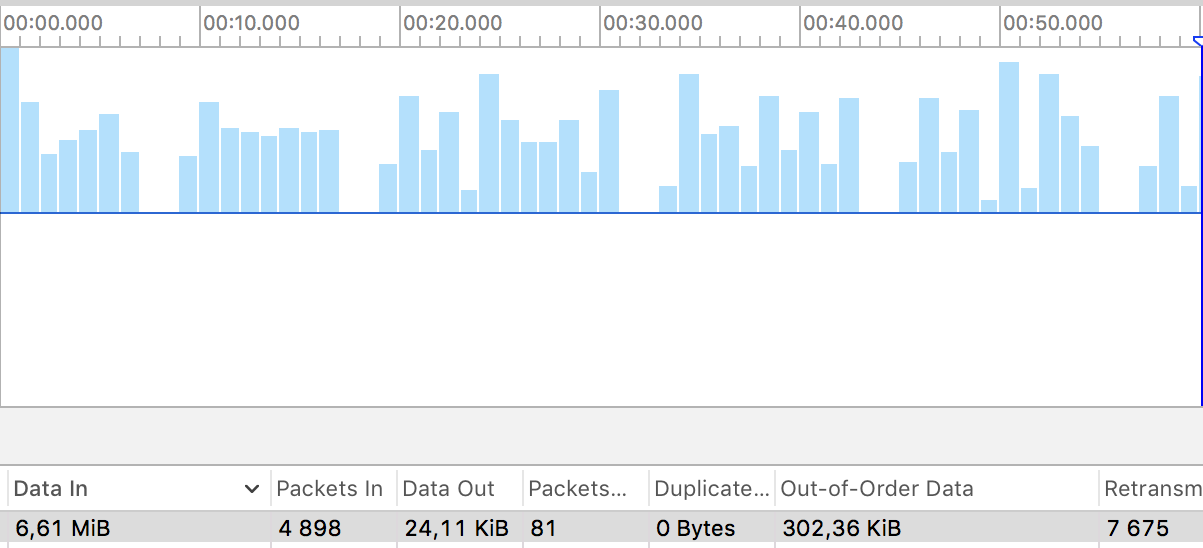
\includegraphics[width=11cm]{networkUsage}
	\caption{Zużycie sieci podczas streamu}
\end{figure}
Przeprowadzono także test na zużycie pamięci RAM i zużycie procesora. Te jednak są niewielkie i wynoszą odpowiednio 25MB pamięci RAM i średnio 1 procent zużycia procesora.
Zużycie procesora wzrasta do poziomu ok. 15 procent tylko w momencie pobierania nagranego obrazu z serwera. Wtedy też zużycie pamięci RAM jest o około 5MB większe i wynosi około 30MB.
\begin{figure}[h]
	\centering
	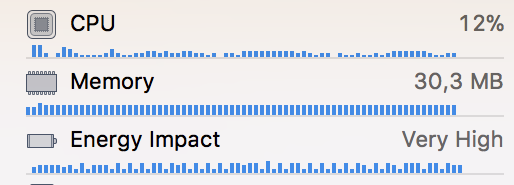
\includegraphics[width=11cm]{CPURAM}
	\caption{Zużycie procesora i RAM podczas największego obciążenia}
\end{figure}
Testy przeprowadzono na iPhonie 6S i iPadzie Pro.




\section*{Aplikacja internetowa}
Aplikacja webowa przeznaczona jest dla użytkowników wszystkich systemów operacyjnych i~została przetestowana w~przeglądarce Firefox. Rozmieszczenie komponentów aplikacji różni się od tego zastosowanego w~aplikacjach IOS oraz Android - spowodowane jest to inną rozdzielczością ekranu. 

\paragraph{Panel logowania / rejestracji użytkownika:}
\paragraph{Menu wyboru urządzenia:}
\paragraph{Główny panel aplikacji:}
\paragraph{Panel rejestracji urządzenia:}
\paragraph{Panel notyfikacji:}


\paragraph{Implementacja Django - połączenie z bazą danych:}
Biblioteka Django posiada wbudowane rozwiązania umożliwiające pobieranie informacji z bazy danych projektu dzięki czemu aplikacja webowa nie wysyła zapytań na określone dla aplikacji mobilnych porty, tylko komunikuje się bezpośrednio z bazą danych. Rozwiązanie to umożliwia uniezależnienie aplikacji webowej od stanu portów oraz zmniejsza liczbę potrzebnych zapytań wysyłanych do serwera.